\section{Mixture-of-Experts at Frontier Scale}

\begin{frame}{}
    \LARGE Next-Generation Architectures: \textbf{Mixture-of-Experts}

    \vspace{1em}
    \normalsize Must every token use every weight?
\end{frame}

\begin{frame}{MoE in One Slide (Recap)}
    \begin{columns}[T,onlytextwidth]
        \column{0.55\textwidth}
        \begin{itemize}\itemsep0.5em
            \item In GPT-3, the feed-forward layers hold 116B of 175B parameters, about \textbf{two thirds}.
            \item MoE replaces one large FFN with $N$ small \emph{experts}. A \textbf{router} sends each token to only $k$ of them:
            \[
                y=\sum_{i\in \mathrm{TopK}(x)} g_i(x)\,\mathrm{FFN}_i(x)
            \]
            \item \textbf{Memory} scales with total parameters. \textbf{Compute} scales with active parameters.
        \end{itemize}
        \column{0.42\textwidth}
        \centering
        \begin{adjustbox}{max width=\linewidth}\begin{tikzpicture}[font=\scriptsize, >=Stealth,
            ex/.style={draw, rounded corners=1.5pt, minimum width=0.85cm, minimum height=0.6cm}]
            \node[draw, rounded corners=1.5pt, fill=gray!12, minimum width=1.4cm, minimum height=0.5cm] (x) at (2.1,0) {token $x$};
            \node[draw, rounded corners=1.5pt, fill=KAUSTcyan!25, minimum width=1.4cm, minimum height=0.5cm] (r) at (2.1,1.0) {\textbf{Router}};
            \node[ex, fill=gray!10] (e1) at (0.3,2.3) {$E_1$};
            \node[ex, fill=darkorange!35] (e2) at (1.5,2.3) {$E_2$};
            \node[ex, fill=gray!10] (e3) at (2.7,2.3) {$E_3$};
            \node[ex, fill=darkorange!35] (e4) at (3.9,2.3) {$E_4$};
            \node[draw, circle, inner sep=1.5pt] (s) at (2.1,3.5) {$+$};
            \draw[->, thick] (x) -- (r);
            \draw[->, thick, darkorange!80!black] (r) -- (e2);
            \draw[->, thick, darkorange!80!black] (r) -- (e4);
            \draw[->, gray!50, dashed] (r) -- (e1);
            \draw[->, gray!50, dashed] (r) -- (e3);
            \draw[->, thick, darkorange!80!black] (e2) -- (s);
            \draw[->, thick, darkorange!80!black] (e4) -- (s);
            \node[gray] at (2.1,4.0) {weighted sum of 2 of 4 experts};
        \end{tikzpicture}\end{adjustbox}
    \end{columns}
    \src{Parameter split: Gormley and Virtue, CMU 10-423 Lecture 16 (2025), slides 7 to 8. Gate equation after Jiang et al., ``Mixtral of Experts,'' \href{https://arxiv.org/abs/2401.04088}{arXiv:2401.04088}.}
\end{frame}

\begin{frame}{What Changed Since Mixtral}
    \begin{center}
    \small
    \renewcommand{\arraystretch}{1.15}
    \begin{adjustbox}{max width=\linewidth}\begin{tabular}{lcccc}
        \toprule
        \textbf{Model} & \textbf{Total / active} & \textbf{Active share} & \textbf{Experts} & \textbf{Top-$k$} \\
        \midrule
        Mixtral 8x7B (Dec 2023) & 47B / 13B & 28\% & 8 & 2 \\
        DeepSeek-V3 (Dec 2024) & 671B / 37B & 5.5\% & 256 + 1 shared & 8 \\
        Qwen3-235B (Apr 2025) & 235B / 22B & 9.4\% & 128 & 8 \\
        Kimi K2 (Jul 2025) & 1.04T / 32.6B & 3.1\% & 384 + 1 shared & 8 \\
        gpt-oss-120b (Aug 2025) & 116.8B / 5.1B & 4.4\% & 128 & 4 \\
        DeepSeek-V4-Pro (Apr 2026) & 1.6T / 49B & 3.1\% & 384 + 1 shared & 6 \\
        \rowcolor{KAUSTcyan!12} Kimi K3 (2026) & 2.8T / 104B & 3.7\% & 896 + 2 shared & 16 \\
        \bottomrule
    \end{tabular}\end{adjustbox}
    \end{center}
    \begin{itemize}\itemsep0.35em
        \item \textbf{Sparser:} the active share fell from 28\% to between 3 and 5\% in about two and a half years.
        \item \textbf{Finer:} from 8 experts to hundreds. Why? Choosing 2 of 8 gives 28 combinations. Choosing 4 of 16 half-size experts gives 1,820, at the same active size.
    \end{itemize}
    \src{Official configuration files and technical reports of each model. Combination count: Welleck, CMU 11-711 Lecture 21 (2026). Kimi Team, ``Kimi K2: Open Agentic Intelligence,'' \href{https://arxiv.org/abs/2507.20534}{arXiv:2507.20534}.}
\end{frame}

\begin{frame}{Who Chooses? Routing Strategies}
    \begin{center}
    \small
    \renewcommand{\arraystretch}{1.25}
    \begin{adjustbox}{max width=\linewidth}\begin{tabular}{>{\raggedright\arraybackslash}p{3.2cm}>{\raggedright\arraybackslash}p{5.2cm}>{\raggedright\arraybackslash}p{4.6cm}}
        \toprule
        \textbf{Strategy} & \textbf{How it works} & \textbf{Catch} \\
        \midrule
        \rowcolor{KAUSTcyan!12} \textbf{Token choice} (top-$k$) & each token picks its $k$ best experts & load can be very uneven \\
        Expert choice & each expert picks its best tokens & perfect balance, but \alert{leaks future tokens} \\
        Hash routing & fixed map from token id to expert & no learning at all \\
        Soft MoE & experts process weighted mixes of tokens & not causal \\
        \bottomrule
    \end{tabular}\end{adjustbox}
    \end{center}
    \begin{itemize}\itemsep0.4em
        \item For a decoder the choice is forced. If an expert chooses among the tokens of a sequence, each decision depends on \emph{later} tokens.
        \item So almost every LLM uses \textbf{token choice}, and must then solve load balancing separately.
        \item Old ideas return: DeepSeek-V4 uses \emph{hash routing} in its first three layers.
    \end{itemize}
    \src{Hashimoto, Stanford CS336 Lecture 4 (2026). Zhou et al., \href{https://arxiv.org/abs/2202.09368}{arXiv:2202.09368}. Wang et al., \href{https://arxiv.org/abs/2408.15664}{arXiv:2408.15664}. Puigcerver et al., \href{https://arxiv.org/abs/2308.00951}{arXiv:2308.00951}. DeepSeek-V4 report, \href{https://arxiv.org/abs/2606.19348}{arXiv:2606.19348}.}
\end{frame}

\begin{frame}{The Gate: From Softmax to Sigmoid}
    \begin{columns}[T,onlytextwidth]
        \column{0.48\textwidth}
        \textbf{Softmax gate} (Mixtral, Qwen3, gpt-oss)
        \[
            g = \mathrm{Softmax}\big(\mathrm{TopK}(x W_g)\big)
        \]
        \begin{itemize}\itemsep0.3em
            \item Experts \emph{compete}. Raising one score lowers the others.
        \end{itemize}
        \column{0.5\textwidth}
        \textbf{Sigmoid gate} (DeepSeek-V3, Kimi, GLM)
        \[
            s_i=\sigma(x^\top e_i), \qquad g_i=\frac{s_i}{\sum_{j\in \mathrm{TopK}} s_j}
        \]
        \begin{itemize}\itemsep0.3em
            \item Each expert is scored \emph{on its own}, then the selected scores are normalised.
        \end{itemize}
    \end{columns}
    \vspace{0.6em}
    \begin{itemize}\itemsep0.45em
        \item Sigmoid scoring pairs naturally with the bias-based balancing on the next slide. DeepSeek-V3, Kimi K2 and K3, and GLM-5 all use the pair.
        \item \textbf{2026:} DeepSeek-V4 changes the score again, to $\sqrt{\mathrm{softplus}(\cdot)}$. The report gives no ablation for it.
    \end{itemize}
    \src{Jiang et al., \href{https://arxiv.org/abs/2401.04088}{arXiv:2401.04088}. DeepSeek-AI, ``DeepSeek-V3 Technical Report,'' \href{https://arxiv.org/abs/2412.19437}{arXiv:2412.19437}. DeepSeek-V4, \href{https://arxiv.org/abs/2606.19348}{arXiv:2606.19348}. Configuration files of Qwen3, gpt-oss, Kimi K2, Kimi K3 and GLM-5.}
\end{frame}

\begin{frame}{Balancing Without an Auxiliary Loss}
    \begin{columns}[T,onlytextwidth]
        \column{0.54\textwidth}
        \begin{itemize}\itemsep0.45em
            \item \textbf{The dilemma.} A \emph{balance loss} is an extra training term that penalises uneven use of the experts. It fights the language-modelling loss. Too weak: experts collapse. Too strong: quality drops.
            \item \textbf{The fix.} Add a per-expert bias $b_i$ that is used \emph{only to select}:
            \[
                i \in \mathrm{TopK}\big(\{s_j + b_j\}\big), \qquad g_i \text{ still from } s_i
            \]
            \item After each step, nudge $b_i$ up for underloaded experts and down for overloaded ones.
            \item No gradient ever flows from the balancing rule into the model.
        \end{itemize}
        \column{0.44\textwidth}
        \centering
        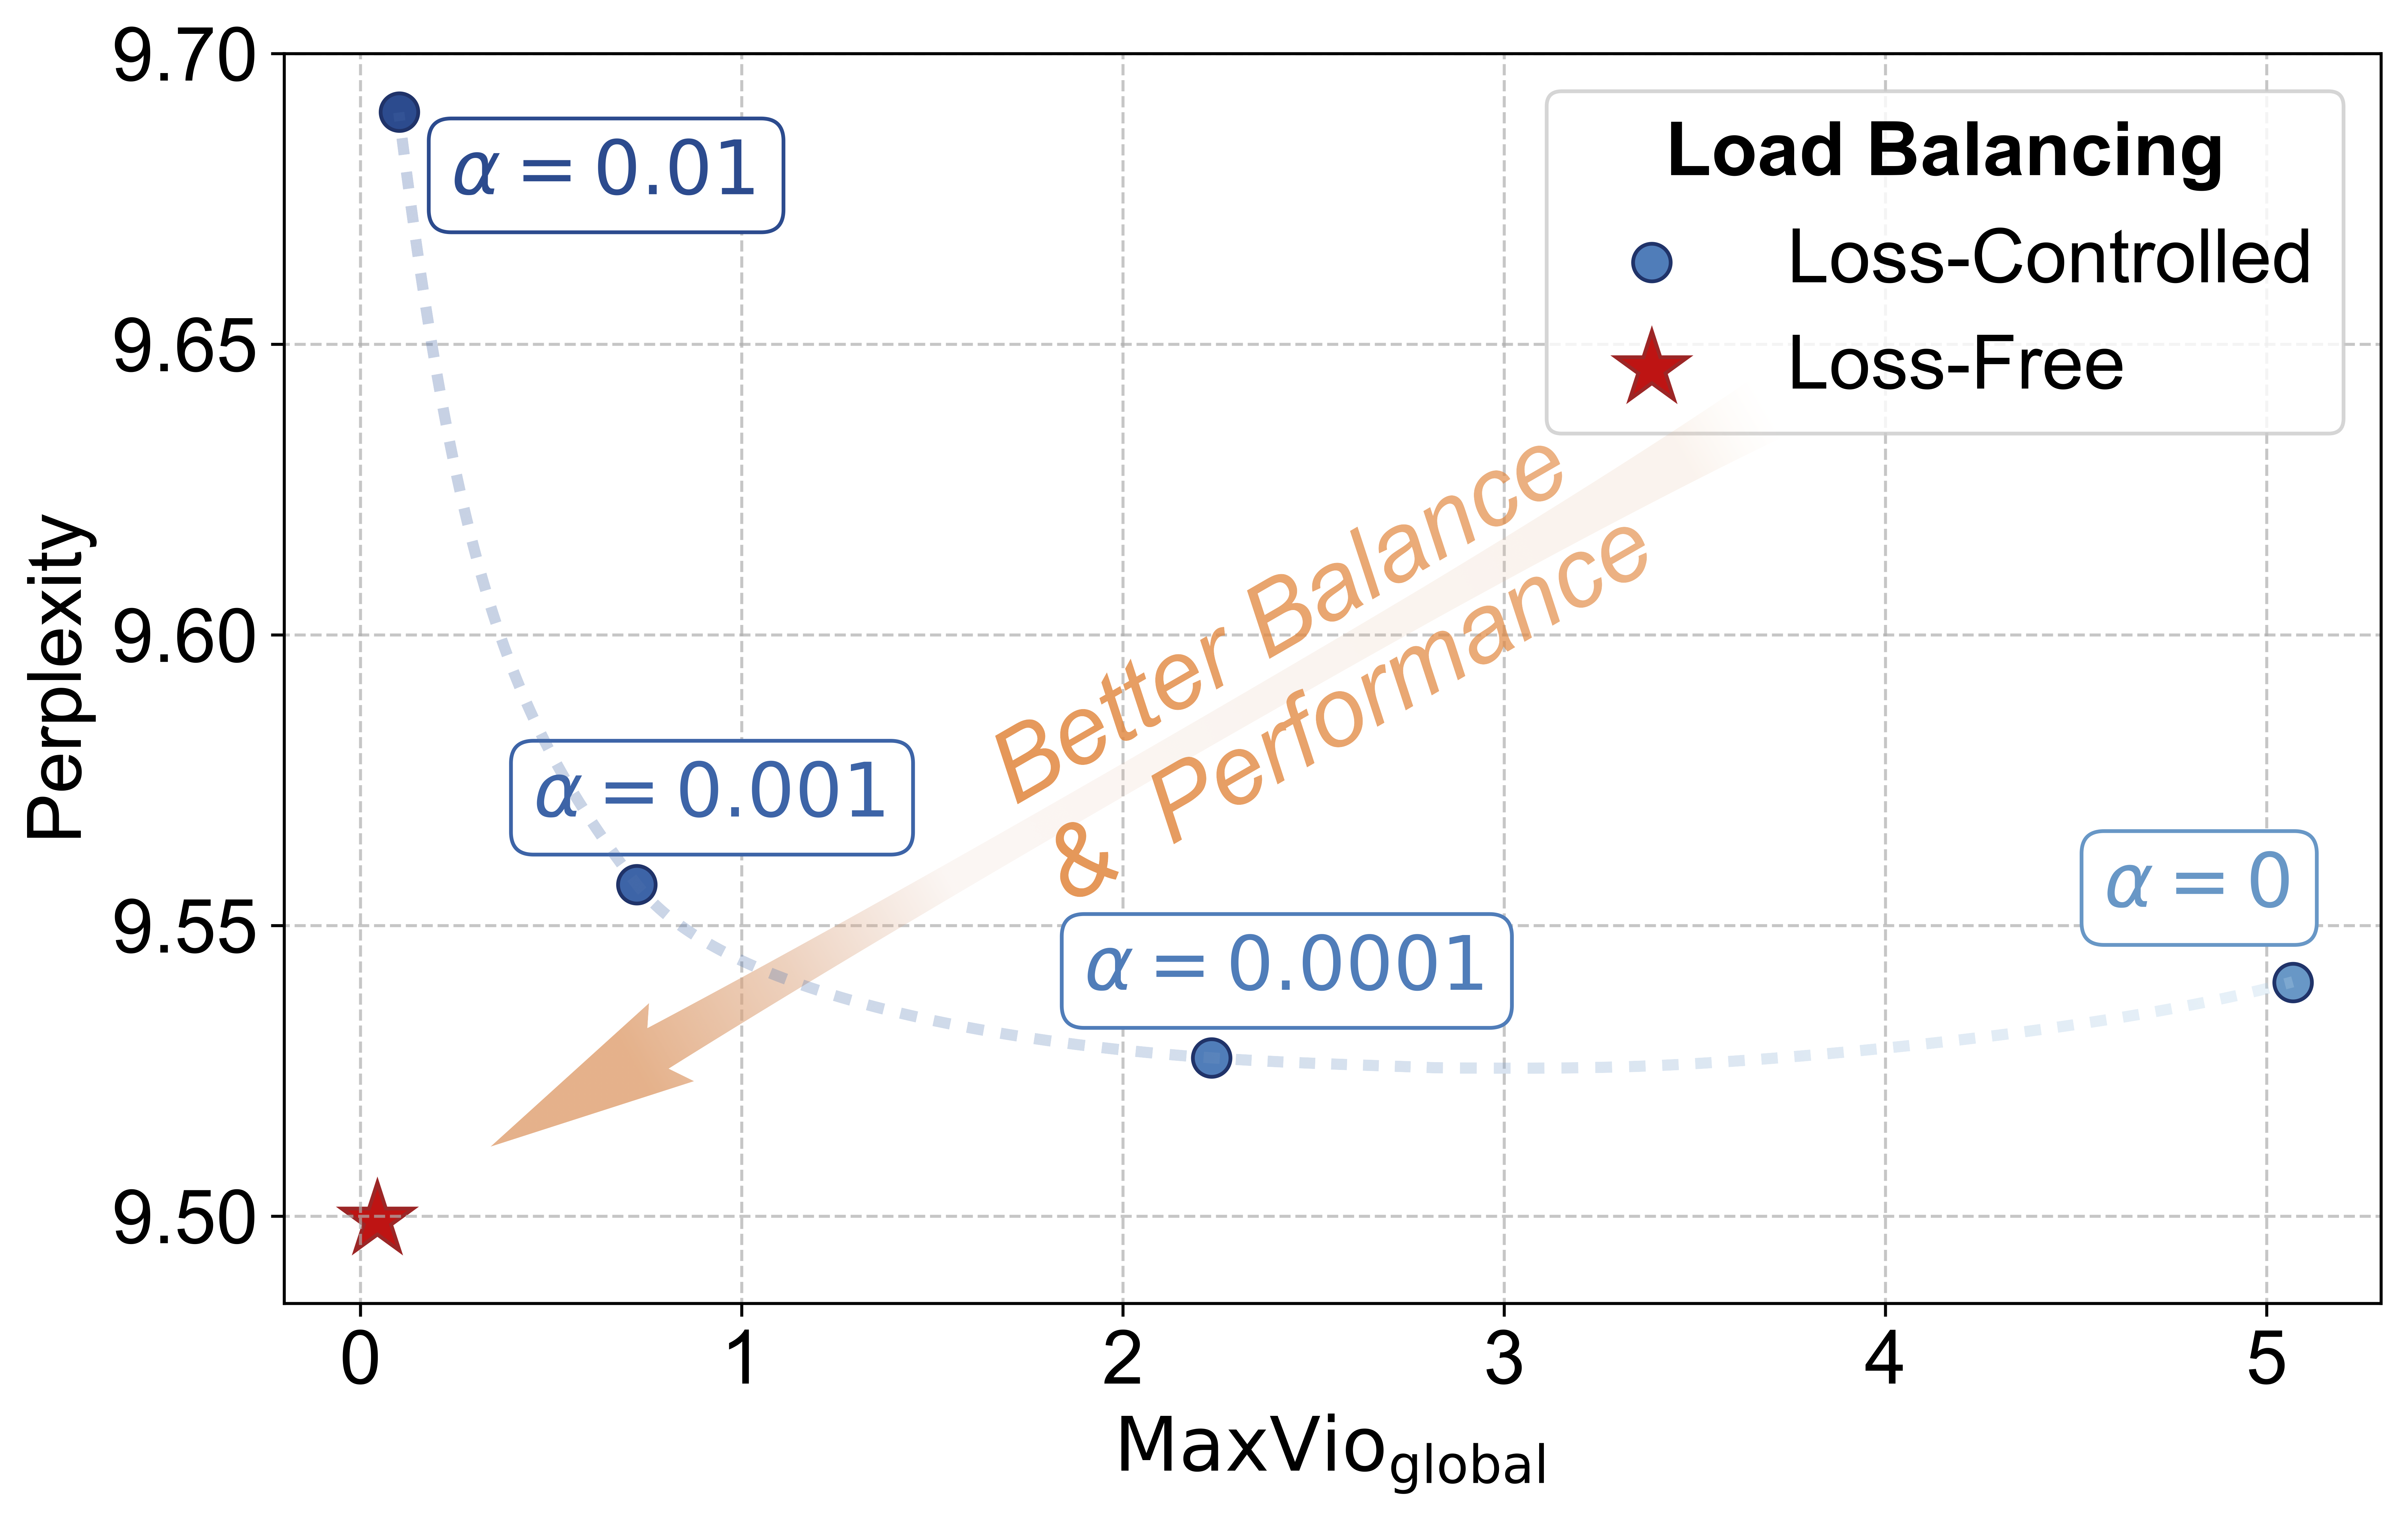
\includegraphics[width=\linewidth,height=0.55\textheight,keepaspectratio]{images/next-gen-architectures/auxfree_fig2_dilemma.png}
    \end{columns}
    \vspace{0.2em}
    \src{Wang et al., ``Auxiliary-Loss-Free Load Balancing Strategy for Mixture-of-Experts,'' \href{https://arxiv.org/abs/2408.15664}{arXiv:2408.15664}, Figure 2. $\mathrm{MaxVio}$ measures how far the busiest expert is above the mean load.}
\end{frame}

\begin{frame}{The Real Lesson: Balance the Batch, Not the Sequence}
    \begin{itemize}\itemsep0.4em
        \item Why did the bias method help? DeepSeek's own control experiment gives a surprising answer.
    \end{itemize}
    \begin{center}
    \small
    \begin{adjustbox}{max width=\linewidth}\begin{tabular}{lcc}
        \toprule
        \textbf{Validation loss} & \textbf{1B model} & \textbf{3B model} \\
        \midrule
        Auxiliary loss, balanced per \emph{sequence} & 2.258 & 2.085 \\
        Auxiliary loss, balanced per \emph{batch} & 2.253 & 2.080 \\
        Bias method (no auxiliary loss) & 2.253 & 2.080 \\
        \bottomrule
    \end{tabular}\end{adjustbox}
    \end{center}
    \begin{itemize}\itemsep0.4em
        \item The \textbf{scope} matters more than the method. Forcing every sequence to use all experts evenly stops experts from specialising. A code file \emph{should} favour code experts.
        \item Qwen reached the same conclusion from the other side. Computing the balance loss over a \textbf{global batch} lifted a 43B model from 54.98 to 57.30 on MMLU.
        \item Note: frontier models still keep a very small sequence-level loss as a safety net.
    \end{itemize}
    \src{DeepSeek-AI, \href{https://arxiv.org/abs/2412.19437}{arXiv:2412.19437}, Section 4.5.3. Qiu et al., ``Demons in the Detail: On Implementing Load Balancing Loss for Training Specialized Mixture-of-Expert Models,'' \href{https://arxiv.org/abs/2501.11873}{arXiv:2501.11873}, Table 1.}
\end{frame}

\begin{frame}{Do Experts Specialise? An Updated Answer}
    \centering
    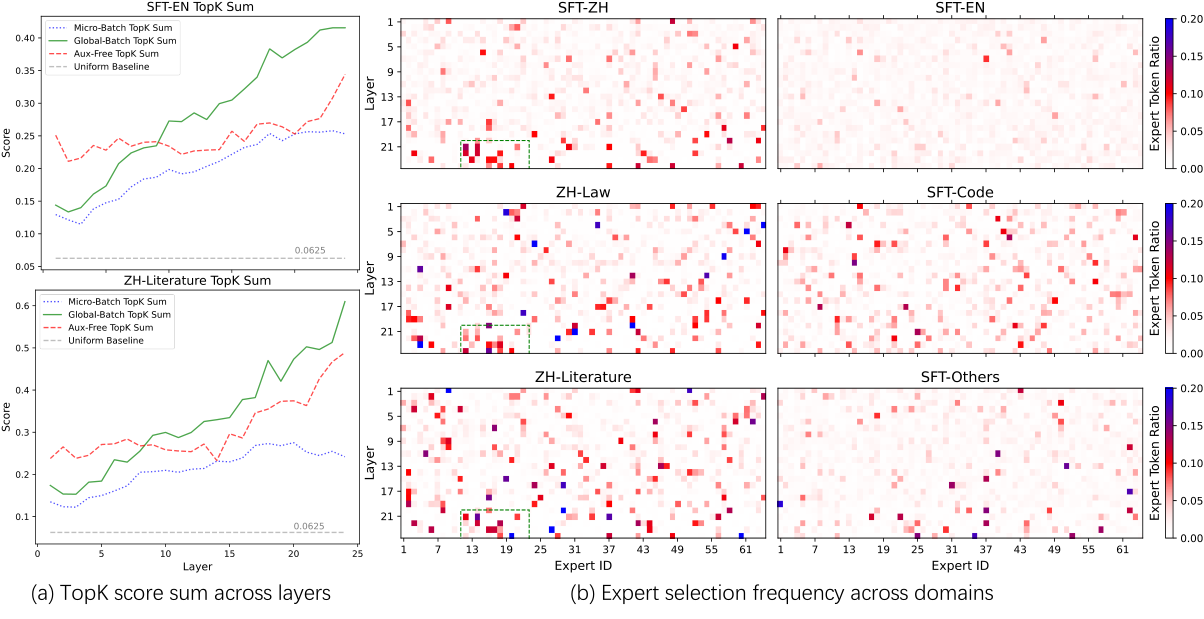
\includegraphics[width=0.95\linewidth,height=0.52\textheight,keepaspectratio]{images/next-gen-architectures/qwen_global_lbl_fig.png}
    \begin{itemize}\itemsep0.2em
        \item \textbf{2024 answer (Mixtral):} no clear domain specialisation. arXiv, biology and philosophy text route alike.
        \item \textbf{2025 answer:} it depends on training. With batch-level balancing, domain experts appear (above, right). OLMoE, trained from scratch, shows the same.
    \end{itemize}
    \src{Figure: Qiu et al., \href{https://arxiv.org/abs/2501.11873}{arXiv:2501.11873}. Jiang et al., \href{https://arxiv.org/abs/2401.04088}{arXiv:2401.04088}, Section 5. Muennighoff et al., ``OLMoE: Open Mixture-of-Experts Language Models,'' \href{https://arxiv.org/abs/2409.02060}{arXiv:2409.02060}.}
\end{frame}

\begin{frame}{The Router Is Fragile: Stability and Token Dropping}
    \begin{itemize}\itemsep0.33em
        \item Router logits pass through an exponential. In bfloat16, large logits mean large round-off, and training diverges.
        \item \textbf{Router z-loss} keeps the logits small:
        \[
            L_z=\frac1B\sum_{i=1}^{B}\Big(\log\sum_{j=1}^{N}e^{x^{(i)}_j}\Big)^2
        \]
        \item The habit survives in 2026. Experts are stored in \textbf{4-bit} formats, while routers stay in higher precision.
        \item \textbf{Token dropping.} Early MoEs gave each expert a fixed capacity and dropped the overflow. Another user's request could cost you a token.
        \item Modern training is \textbf{dropless}. Block-sparse kernels let each expert take any number of tokens, and DeepSeek-V3 drops none in training or inference.
    \end{itemize}
    \src{Zoph et al., ``ST-MoE: Designing Stable and Transferable Sparse Expert Models,'' \href{https://arxiv.org/abs/2202.08906}{arXiv:2202.08906}. Gale et al., ``MegaBlocks,'' \href{https://arxiv.org/abs/2211.15841}{arXiv:2211.15841}. DeepSeek-AI, \href{https://arxiv.org/abs/2412.19437}{arXiv:2412.19437}. Hashimoto, Stanford CS336 Lecture 4 (2026).}
\end{frame}

\begin{frame}{JetMoE: Sparsity in Attention Too}
    \begin{columns}[T,onlytextwidth]
        \column{0.68\textwidth}
        \begin{itemize}\itemsep0.5em
            \item \textbf{Question:} if routing works for the FFN, why not for attention heads?
            \item \textbf{Design:} every layer routes twice. Top-2 of 8 \emph{attention experts}, then top-2 of 8 \emph{MLP experts}. Keys and values are shared. Each attention expert owns its query and output projections.
            \item \textbf{Result:} 8B total, about 2B active. Trained on 1.25T tokens for \alert{under \$0.1M}, and it beat Llama-2-7B on the Open LLM average (53.0 against 51.0).
            \item \textbf{Why it matters:} 30,000 H100 GPU-hours is a budget a university lab can reach.
            \item \textbf{What did not transfer:} none of the frontier configurations in this lecture routes its attention heads. Attention sparsity took a different road, which we meet in the next section.
        \end{itemize}
        \column{0.28\textwidth}
        \centering
        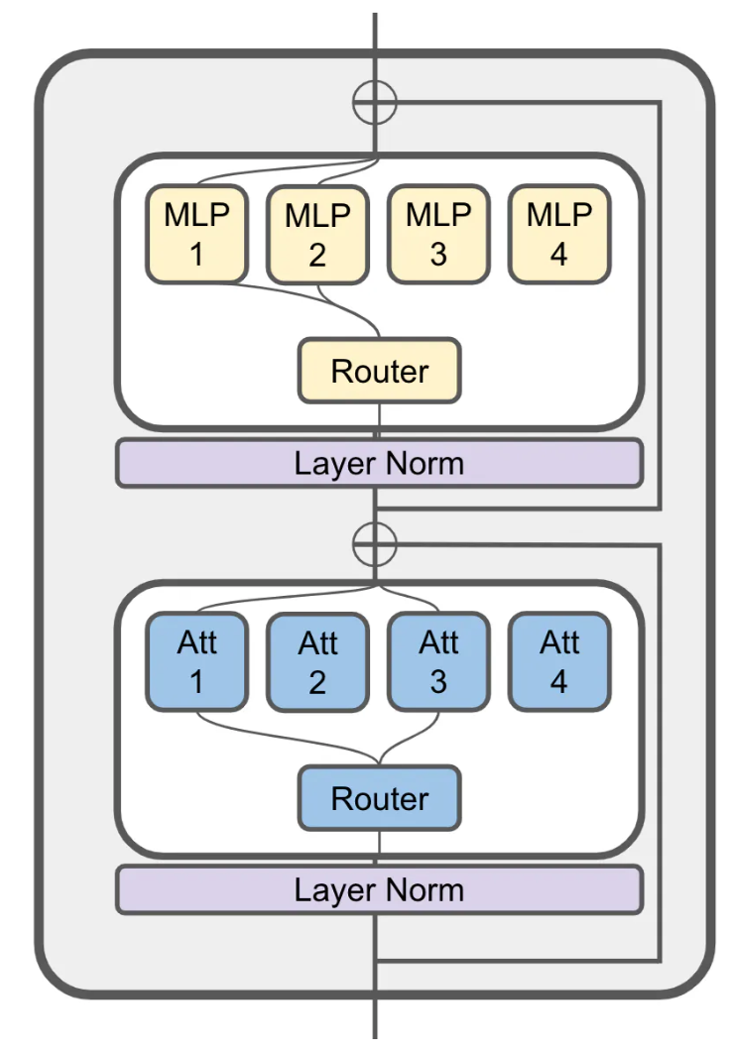
\includegraphics[width=\linewidth,height=0.66\textheight,keepaspectratio]{images/next-gen-architectures/jetmoe_fig1_architecture.png}
    \end{columns}
    \src{Shen et al., ``JetMoE: Reaching Llama2 Performance with 0.1M Dollars,'' \href{https://arxiv.org/abs/2404.07413}{arXiv:2404.07413}, Figure 1 and Table 3.}
\end{frame}

\begin{frame}{Scaling Laws for MoE}
    \begin{itemize}\itemsep0.5em
        \item \textbf{How fine should experts be?} Define granularity $G = d_{\text{ff}} / d_{\text{expert}}$. The fitted law
        \[
            \mathcal{L}(N,D,G)=c+\Big(\frac{g}{G^{\gamma}}+a\Big)\frac{1}{N^{\alpha}}+\frac{b}{D^{\beta}}
        \]
        says the compute-optimal $G$ \textbf{grows with scale}, and $G=1$ is almost never optimal.
        \item \textbf{How sparse?} At fixed compute, sparser is better, and the optimal sparsity approaches 1 as models grow.
        \item \textbf{The warning.} At matched loss, sparser models do \alert{worse on reading comprehension}. Loss does not tell the whole story.
    \end{itemize}
    \vspace{0.2em}
    \takeaway{An old rule is dead: ST-MoE (2022) found the benefit ``quickly diminishes'' beyond 256 experts. Kimi K3 uses 896.}
    \src{Krajewski et al., ``Scaling Laws for Fine-Grained Mixture of Experts,'' \href{https://arxiv.org/abs/2402.07871}{arXiv:2402.07871}. Abnar et al., \href{https://arxiv.org/abs/2501.12370}{arXiv:2501.12370}. ``Hyperparameter Scaling Laws Across MoE Sparsity,'' \href{https://arxiv.org/abs/2609.08690}{arXiv:2609.08690}.}
\end{frame}

\begin{frame}{Serving a Trillion-Parameter MoE}
    \begin{itemize}\itemsep0.3em
        \item \textbf{MoE is a throughput play at large batch.} At batch size 1 you pay memory for every expert and save only FLOPs.
        \item \textbf{Expert parallelism.} Experts live on different GPUs, so every MoE layer is an all-to-all exchange of tokens. DeepSeek serves V3 with experts spread over 144 GPUs in decode.
        \item \textbf{The batch must be large.} With 8 of 256 experts active, each expert sees few tokens unless many requests are pooled. In SGLang's tests, overlapping two batches in decode pays off only above 64 to 128 tokens per device.
        \item \textbf{Low-bit experts.} Experts are most of the weights, and each is used rarely. gpt-oss stores them at 4.25 bits per parameter, so the 120B model fits on one 80 GB GPU.
        \item \textbf{Co-design.} \emph{LatentMoE} (NVIDIA, Kimi K3) projects each token to a smaller latent space before dispatch, and the experts compute there. The smaller payload pays for more experts and a larger top-$k$.
    \end{itemize}
    \src{DeepSeek, ``DeepSeek-V3/R1 Inference System Overview'' (2025). SGLang team, large-scale expert parallelism blog (May 2025). OpenAI, gpt-oss model card, \href{https://arxiv.org/abs/2508.10925}{arXiv:2508.10925}. ``LatentMoE,'' \href{https://arxiv.org/abs/2601.18089}{arXiv:2601.18089}.}
\end{frame}

\begin{frame}{MoE: What to Remember}
    \begin{itemize}\itemsep0.6em
        \item The newest frontier MoEs activate \textbf{3 to 5\%} of their weights per token, across hundreds of small experts.
        \item Routing is \textbf{token choice}, because a decoder must stay causal.
        \item Balancing moved from a loss term to a \textbf{selection bias}, and from the sequence to the \textbf{batch}. That shift is what lets experts specialise.
        \item The router is the delicate part: keep its logits small and its precision high.
        \item Open design questions: shared experts, dense early layers, and the right score function.
    \end{itemize}
    \vspace{0.4em}
    \takeaway{\textbf{Next.} We made the feed-forward block sparse. Can we do the same to attention itself, without giving up exact recall?}
\end{frame}
